\documentclass[12pt]{article}
\usepackage{enumerate}
\usepackage{amsfonts}
\usepackage{amsmath}
\usepackage{fancyhdr}
\usepackage{amsmath}
\usepackage{amssymb}
\usepackage{amsthm}
\usepackage{listings}
\usepackage{mdframed}
\usepackage{graphicx}

\begin{document}
\title{Midterm 2 Version 1 Solution}
\maketitle

\section*{Question 1}
\begin{enumerate}[a.]
    \item

    \begin{align*}
        100 \div 2 = 50,\:&\text{Remainders}\:\textbf{0}\\
        50 \div 2 = 25,\:&\text{Remainders}\:\textbf{0}\\
        25 \div 2 = 12,\:&\text{Remainders}\:\textbf{1}\\
        12 \div 2 = 6,\:&\text{Remainders}\:\textbf{0}\\
        6 \div 2 = 3,\:&\text{Remainders}\:\textbf{0}\\
        3 \div 2 = 1,\:&\text{Remainders}\:\textbf{1}\\
        1 \div 2 = 0,\:&\text{Remainders}\:\textbf{1}
    \end{align*}

    \bigskip

    Then, it follows from above that the binary representation of 100 is $(1100100)_2$.

    \item The smallest number that can be expressed by an n-digit balanced ternary
    representation is

    \begin{align}
        \sum\limits_{i=0}^{n-1} d_i \cdot 3^i,\:\text{where}\:d_i \in \{0,1,2\}
    \end{align}

    \bigskip

    \begin{mdframed}
        \underline{\textbf{Correct Solution:}}

        \bigskip

        The smallest number that can be expressed by an n-digit balanced ternary
        representation is

        \setcounter{equation}{0}
        \color{red}
        \begin{align}
            -\left[ \sum\limits_{i=0}^{n-1} 3^i \right]
        \end{align}
        \color{black}
    \end{mdframed}

    \bigskip

    \textbf{Notes:}

    \begin{itemize}
        \item Realized professor is asking for an example of the smallest number.
        \item Ternary representation of a number

        \begin{align*}
            \sum\limits_{i=0}^{n-1} d_i \cdot 3^i,\:\text{where}\:d_i \in \{0,1,2\}
        \end{align*}

        \item Learned a negative number could be expressed in in ternary or binary
        representation of numbers.
    \end{itemize}

    \item

    \begin{tabular}{|c|c|c|c|c|c|}
        \hline
        $f(n) \in \Omega(n)$ & True & $g(n) \in \Omega(n)$ & False & $f(n) \in \mathcal{O}(g(n))$ & False\\
        \hline
        $f(n) \in \Theta(g(n))$ & False & $g(n) \in \Theta(\log_3 n)$ & True & $f(n) + g(n) \in \Theta(f(n))$ & True\\
        \hline
    \end{tabular}

    \bigskip

    \textbf{Notes:}

    \begin{itemize}
        \item

        $\forall g:\mathbb{N} \to \mathbb{R}^{\geq 0}$, and all numbers $a \in \mathbb{R}^{\geq 0}$,
        if $g \in \mathcal{O}(f)$, then $f + g \in \mathcal{O}(f)$

        \item
        $g \in \Theta(f):\: g \in \mathcal{O}(f) \land g \in \Omega(f)$

        or

        $g \in \Theta(f):\:\exists c_1,c_2,n_1 \in \mathbb{R}^{+}, \forall n \in \mathbb{N}, n \geq n_1
        \Rightarrow c_1g(n) \leq f(n) \leq c_2g(n)$, where $f,g:\:\mathbb{N} \to \mathbb{R}^{\geq 0}$

        \item
        $g \in \Omega(f):\:\exists c,n_o \in \mathbb{R}^{+},\:\forall n \in
        \mathbb{N},\:n \geq n_0 \Rightarrow g(n) \geq cf(n)$, where $f,g:\mathbb{N} \to \mathbb{R}^{\geq 0}$

        \item

        $g \in \mathcal{O}(f):\:\exists c,n_o \in \mathbb{R}^{+},\:\forall n \in
        \mathbb{N},\:n \geq n_0 \Rightarrow g(n) \leq cf(n)$, where $f,g:\mathbb{N} \to \mathbb{R}^{\geq 0}$

    \end{itemize}

    \item

    \begin{tabular}{|c|c|c|c|c|}
        \hline
        k & 0 & 1 & 2\\
        \hline
        $i_k$ & $3 = 3^1$ & $9 = 3^2$ & $81 = 3^4$\\
        \hline
    \end{tabular}

    \bigskip

    The value of $i_k$ is
    \setcounter{equation}{0}
    \begin{align}
        3^{2^k}
    \end{align}

    \bigskip

    \textbf{Notes:}

    \begin{itemize}
        \item Realized we are only concerned with the lines \textbf{i = i * i} and \textbf{i = 3}
    \end{itemize}

    \item The number of iterations the function's loop will run is

    \setcounter{equation}{0}
    \begin{align}
        \lceil \log_2 \log_3 n \rceil - 1
    \end{align}

    \textbf{Notes:}

    \begin{itemize}
        \item The loop terminates when $3^{2^{(k+1)}} = i_{k+1} = i_k \cdot i_k \geq n$.
        \item $\forall x \in \mathbb{Z},\:\forall y \in \mathbb{R},\:\lfloor x+y \rfloor = x + \lfloor y \rfloor$
        \item Feel more confident there is no need to add an extra \textbf{+1}. Done by
        playing with examples (i.e is $\lceil \log \log_3 (82) \rceil - 1$ true? Would the loop run only once?)
    \end{itemize}

\end{enumerate}

\section*{Question 2}
\begin{itemize}
    \item

    \textbf{Predicate Logic:} $\forall n \in \mathbb{N}, n \geq 3 \Rightarrow 5^n + 50 < 6^n$

    \bigskip

    \begin{proof}

    Let $n \in \mathbb{N}$.

    \bigskip

    We will prove the statement by induction on $n$.

    \bigskip

    \textbf{Base Case ($n = 3$):}

    \bigskip

    Let $n = 3$.

    \bigskip

    We want to show $5^3 + 50 < 6^3$.

    \bigskip

    Starting from $5^3 + 50$, we can calculate

    \setcounter{equation}{0}
    \begin{align}
        5^3 + 50 &= 125 + 50\\
        &= 175\\
        &< 216\\
        &< 6^3
    \end{align}

    \bigskip

    \textbf{Inductive Case:}

    \bigskip

    Let $n \in \mathbb{N}$. Assume $n \geq 3$ and $5^n + 50 < 6^n$.

    \bigskip

    We want to show $5^{n+1} + 50 < 6^{n+1}$.

    \bigskip

    Starting from $5^{n+1} + 50$, we can calculate

    \begin{align}
        50^{n+1} + 50 &= 5^n \cdot 5 + 50\\
        &< 5^n \cdot 5 + 50 \cdot 5\\
        &< 5(5^n + 50)
    \end{align}

    \bigskip

    Then,

    \begin{align}
        50^{n+1} + 5 &< 5 \cdot 6^n\\
        &< 6 \cdot 6^n\\
        &< 6^{n+1}
    \end{align}

    by using inductive hypothesis (i.e $5^n + 50 < 6^n$)

    \end{proof}

    \bigskip

    \begin{mdframed}
        \underline{\textbf{Correct Solution:}}

        \bigskip

        Let $n \in \mathbb{N}$.

        \bigskip

        We will prove the statement by induction on $n$.

        \bigskip

        \textbf{Base Case ($n = 3$):}

        \bigskip

        Let $n = 3$.

        \bigskip

        We want to show $5^3 + 50 < 6^3$.

        \bigskip

        Starting from $5^3 + 50$, we can calculate

        \setcounter{equation}{0}
        \begin{align}
            5^3 + 50 &= 125 + 50\\
            &= 175\\
            &< 216\\
            &< 6^3
        \end{align}

        \bigskip

        \textbf{Inductive Case:}

        \bigskip

        Let $n \in \mathbb{N}$. Assume $n \geq 3$ and $5^n + 50 < 6^n$.

        \bigskip

        We want to show $5^{n+1} + 50 < 6^{n+1}$.

        \bigskip

        Starting from $5^{n+1} + 50$, we can calculate

        \begin{align}
            50^{n+1} + 50 &= 5^n \cdot 5 + 50\\
            &\color{red}=\color{black} 5^n \cdot 5 + 50 \cdot 5\\
            &< 5(5^n + 50)
        \end{align}

        \bigskip

        Then,

        \begin{align}
            50^{n+1} + 5 &< 5 \cdot 6^n\\
            &< 6 \cdot 6^n\\
            &\color{red}=\color{black} 6^{n+1}
        \end{align}

        by using inductive hypothesis (i.e $5^n + 50 < 6^n$)
    \end{mdframed}

    \bigskip

    \textbf{Notes:}

    \begin{itemize}
        \item Noticed professor uses `\textbf{=}' sign if the expression's value
        remains unchanged from the one before

        \bigskip

        See equation 5 and 6 for example.
    \end{itemize}

\end{itemize}

\section*{Question 3}
\begin{itemize}
    \item

    \textbf{Statement:} $\exists a \in \mathbb{R}^{+}$, $an + 1 \in \Theta(n^3)$

    \bigskip

    \textbf{Negation of Statement:} $\forall a \in \mathbb{R}^{+}$,
    $\forall c_1,c_2,n_0 \in \mathbb{R}^{+}$, $\exists n \in \mathbb{N}$,
    $(n \geq n_0) \land \bigl( (an+1 < c_1n^3) \lor (an+1 > c_2n^3) \bigr)$

    \bigskip

    \begin{proof}

    Let $n = \left\lceil max(n_0, \sqrt{\frac{2a}{c_1}}, \sqrt[3]{\frac{1}{c_1}}) \right\rceil + 1$.

    \bigskip

    We will disprove the statement by showing $n \geq n_0$ and $an+1 < c_1n^3$

    \bigskip

    \textbf{Part 1 (Showing $n \geq n_0$):}

    \bigskip

    Using the fact that $\left\lceil max(n_0, \sqrt{\frac{2a}{c_1}}, \sqrt[3]{\frac{1}{c_1}}) \right\rceil$
    will result in a value greater than or equal to $n_0$, we can calculate

    \setcounter{equation}{0}
    \begin{align}
        n_0 &\leq \left\lceil max(n_0, \sqrt{\frac{2a}{c_1}}, \sqrt[3]{\frac{1}{c_1}}) \right\rceil\\
        &\leq \left\lceil max(n_0, \sqrt{\frac{2a}{c_1}}, \sqrt[3]{\frac{1}{c_1}}) \right\rceil + 1
    \end{align}

    \bigskip

    Then, because we know $n = \left\lceil max(n_0, \sqrt{\frac{2a}{c_1}},
    \sqrt[3]{\frac{1}{c_1}}) \right\rceil + 1$, we can conclude

    \begin{align}
       n_0 &\leq n
    \end{align}

    \end{proof}

    \bigskip

    \textbf{Part 2 (Showing $an+1 < c_1n^3$):}

    \bigskip

    We will prove $an +1 < c_1n^3$ by showing $an < \frac{c_1}{2}n^3$ and
    $1 < \frac{c_1}{2}n^3$, and then combining the two together.

    \bigskip

    For the first inequality, because we know $n = \left\lceil max(n_0,
    \sqrt{\frac{2a}{c_1}}, \sqrt[3]{\frac{1}{c_1}}) \right\rceil + 1 > \sqrt{\frac{2a}{c_1}}$,
    we can conclude

    \begin{align}
        \sqrt{\frac{2a}{c_1}} &< n\\
        \frac{2a}{c_1} &< n^2\\
        a &< \frac{c_1}{2}n^2\\
        an &< \frac{c_1}{2}n^3
    \end{align}

    \bigskip

    For the second inequality, because we know $n = \left\lceil max(n_0,
    \sqrt{\frac{2a}{c_1}}, \sqrt[3]{\frac{1}{c_1}}) \right\rceil + 1 > \sqrt[3]{\frac{1}{c_1}}$,
    we can conclude

    \begin{align}
        \sqrt[3]{\frac{1}{c_1}} &< n\\
        \frac{1}{c_1} &< n^3\\
        1 &< n^3
    \end{align}

    \bigskip

    Then,

    \begin{align}
        an +1 &< \frac{c_1}{2} \cdot n^3 + \frac{c_1}{2} \cdot n^3\\
        an + 1 &< c_1n^3
    \end{align}

    \bigskip

    \textbf{Notes:}

    \begin{itemize}
        \item I struggled on this question.
        \item Learned \textbf{+1} in $\left\lceil max(n_0, \sqrt{\frac{2a}{c_1}},
        \sqrt[3]{\frac{1}{c_1}}) \right\rceil + 1 > \sqrt[3]{\frac{1}{c_1}}$ is
        to allow the use of inequality sign `$<$'.
        \item Learned that when $c_1$ is in inequality, with multiple terms like
        $an + 1$ on the other side, and is asking to disprove it, I should first
        divide them up, find valid n for each term, and then recombine
        to create a valid $n$.

        \bigskip

        See figure 1 for example

        \begin{figure}
            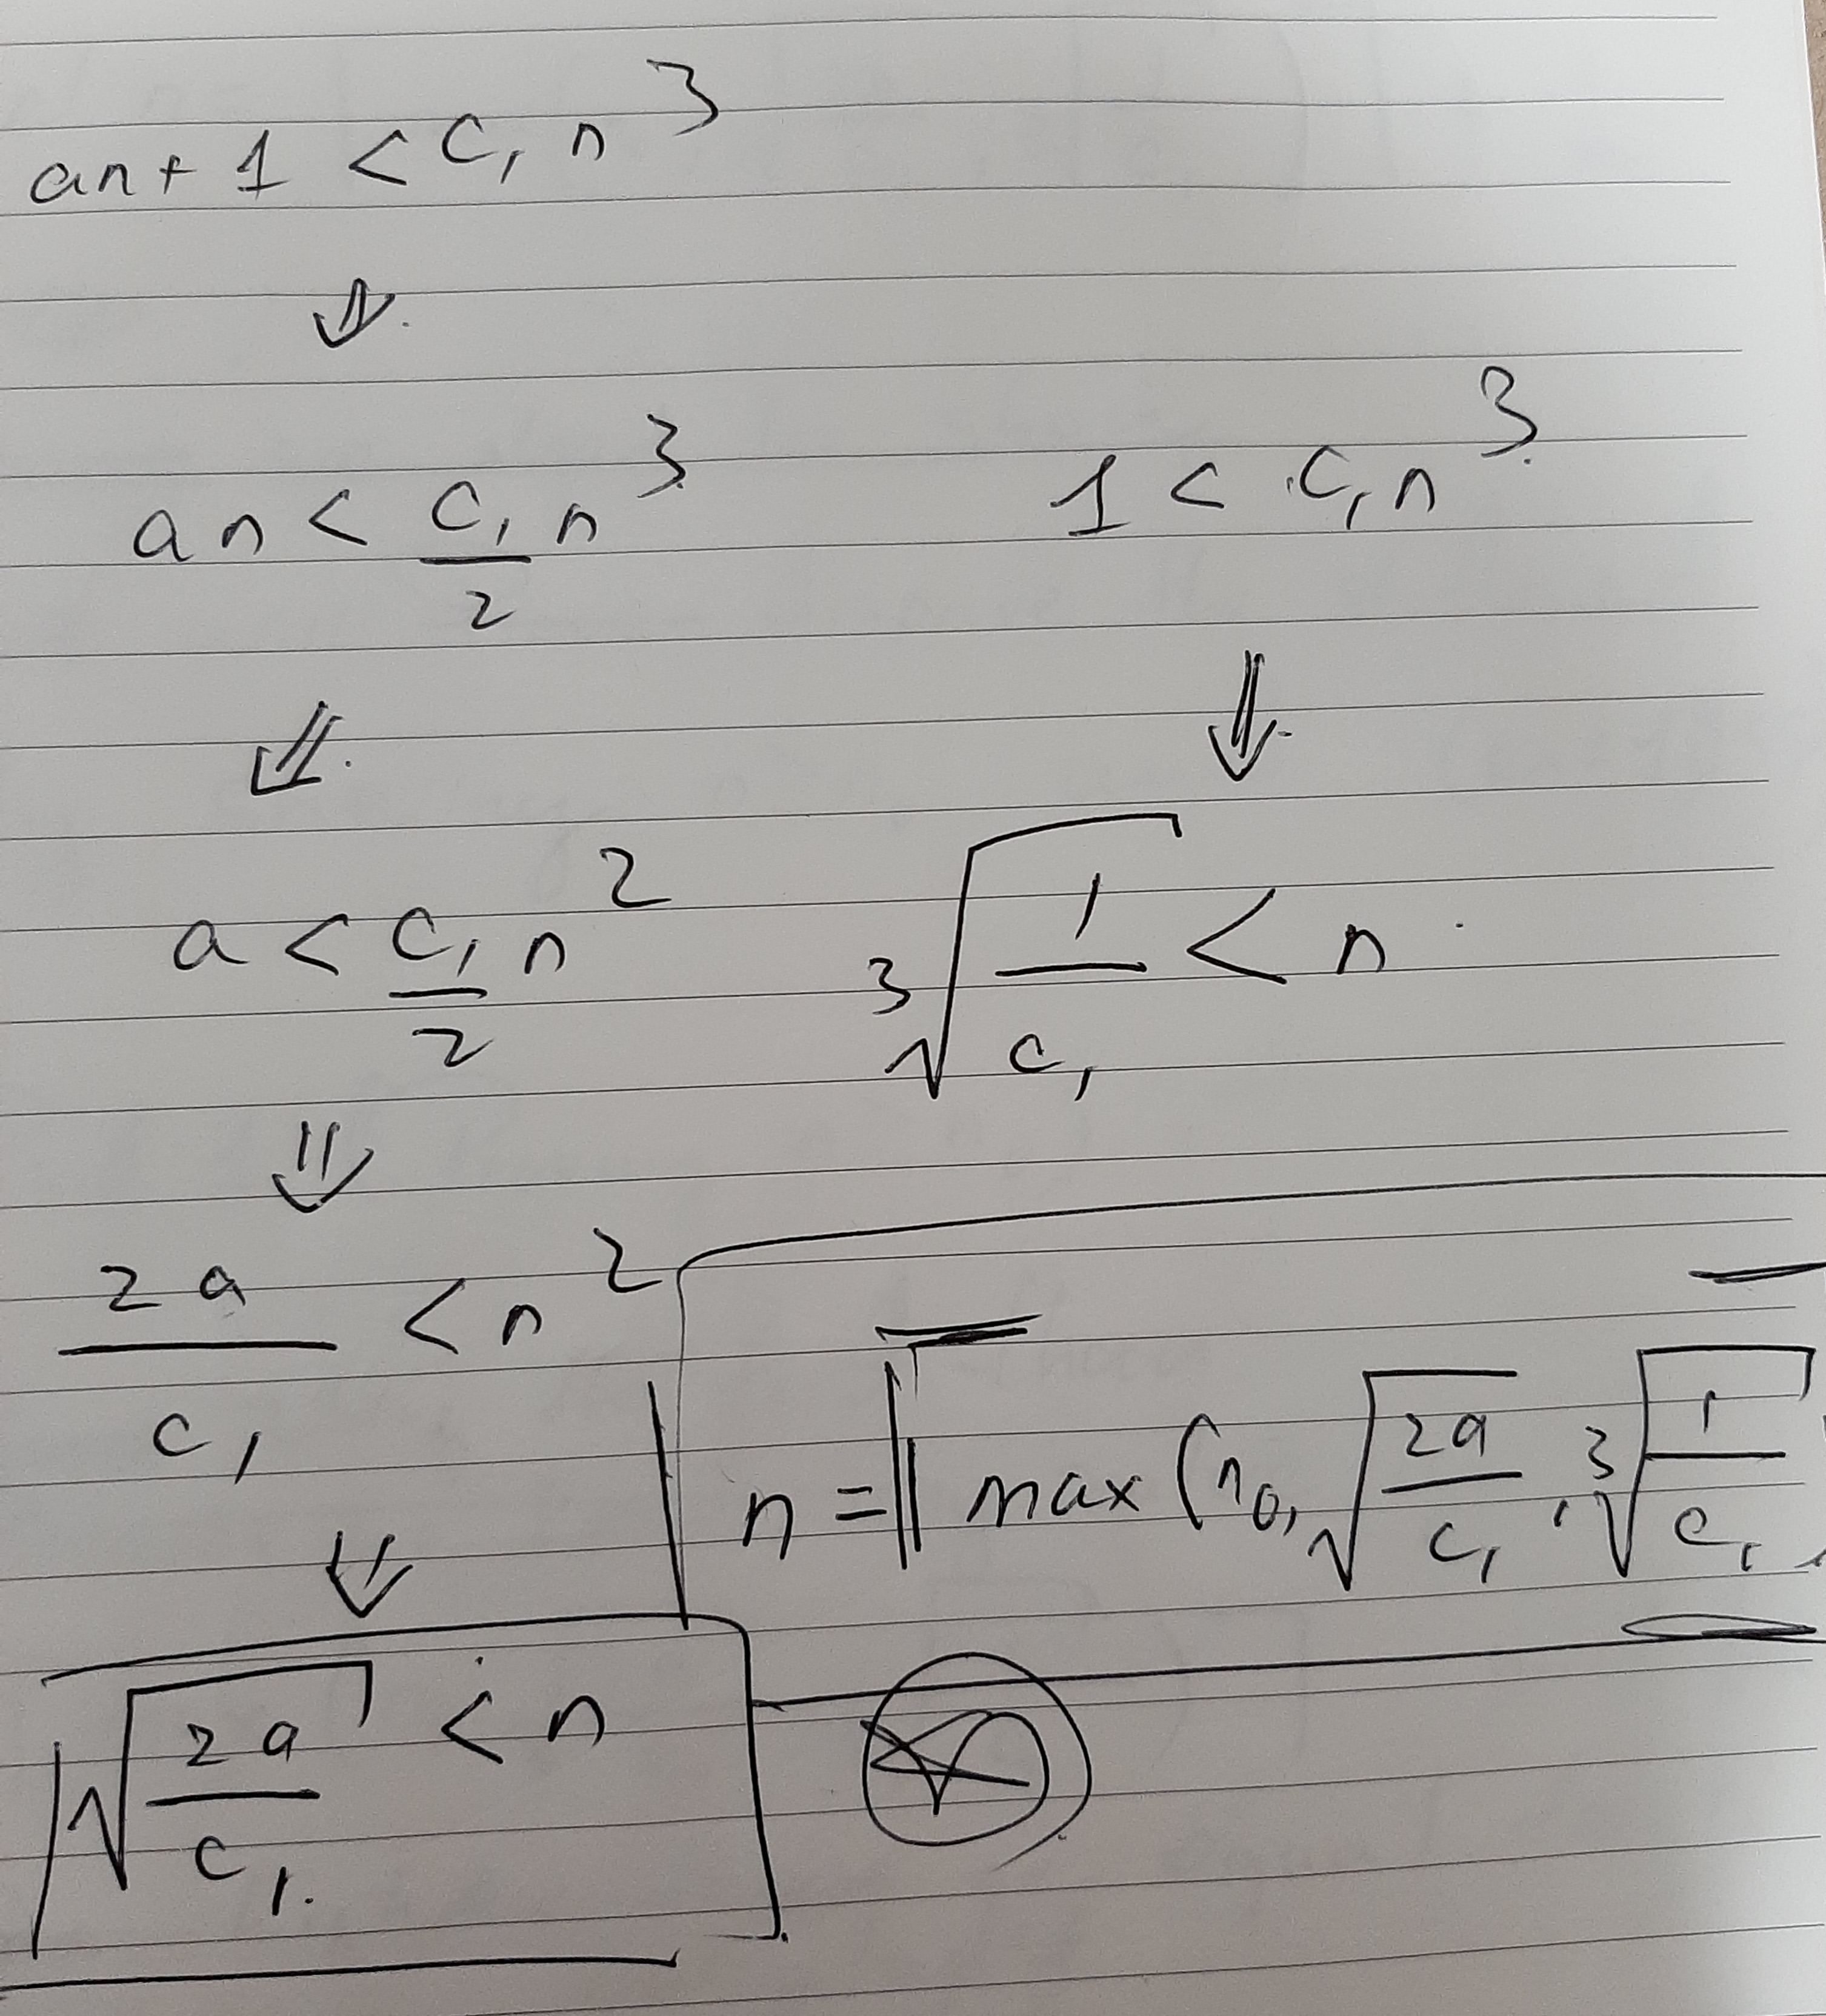
\includegraphics[width=\linewidth]{images/midterm_1_v1_q3_comment.jpg}
            \caption{A sample work for question 3}
        \end{figure}
    \end{itemize}
\end{itemize}

\newpage

\section*{Question 4}

\end{document}